% Homework Assignment Article
% LaTeX Template
\documentclass[a4paper,11pt]{article} 

%----------------------------------------------------------------------------------------
%	FORMATTING
%----------------------------------------------------------------------------------------
\usepackage[a4paper, margin=2.5cm]{geometry}
\setlength{\parskip}{0.5em}
\setlength{\parindent}{0in}

%----------------------------------------------------------------------------------------
%	PACKAGES AND OTHER DOCUMENT CONFIGURATIONS
%----------------------------------------------------------------------------------------
\usepackage[utf8]{inputenc} 
\usepackage[T1]{fontenc}
\usepackage{lmodern}
\usepackage[english, spanish]{babel} 
\usepackage{charter} 
\usepackage{microtype} 
\usepackage{amsthm, amsmath, amssymb} 
\usepackage{float} 
\usepackage[final, colorlinks = true, linkcolor = headerBlue, citecolor = headerBlue, urlcolor = headerBlue]{hyperref} 
\usepackage{graphicx, multicol} 
\usepackage{xcolor} 
\usepackage{colortbl} 
\usepackage{array} 
\usepackage{listings} 
\usepackage{booktabs} 

% Configuración de listings
\lstset{
    language=Java,         
    basicstyle=\ttfamily\small,    
    keywordstyle=\color{blue!70!black}\bfseries,
    commentstyle=\color{green!50!black}\itshape,
    numbers=left,            
    frame=lines             
}

% Configuración TikZ
\usepackage{tikz}
\usetikzlibrary{arrows.meta,positioning,fit,backgrounds,calc,shadows} 

\usepackage{fancyhdr} 
\pagestyle{fancy} 
\fancyhead{}\renewcommand{\headrulewidth}{0pt} 
\fancyfoot[L]{} 
\fancyfoot[C]{} 
\fancyfoot[R]{\thepage} 

%----------------------------------------------------------------------------------------
%	UML DIAGRAM CONFIGURATION
%----------------------------------------------------------------------------------------
\definecolor{headerBlue}{HTML}{245C99} 
\definecolor{headerGreen}{HTML}{2D7A4C} 
\definecolor{assocColor}{HTML}{444444} 
\definecolor{inheritColor}{HTML}{222222}

\newcolumntype{L}[1]{>{\raggedright\arraybackslash}p{#1}}

% UML class macro
\newcommand{\umlclass}[7]{%
  \node[inner sep=0pt, outer sep=0pt, drop shadow={opacity=0.25, shadow xshift=2pt, shadow yshift=-2pt}] (#1) at #2 {%
    \scriptsize\sffamily
    \renewcommand{\arraystretch}{1.25}%
    \setlength{\tabcolsep}{6pt}%
    \begin{tabular}{|L{#3}|}
      \hline
      \rowcolor{#4}\multicolumn{1}{|c|}{\textcolor{white}{\bfseries #5}}\\
      \hline
      \rowcolor{white} #6\\
      \hline
      \rowcolor{white} #7\\
      \hline
    \end{tabular}%
  };%
}

\begin{document}

%----------------------------------------------------------------------------------------
%	TITLE SECTION
%----------------------------------------------------------------------------------------

\title{Documentación Técnica: Actividad 4\\ \large Excepciones, Interfaces Gráficas y Lectura de Archivos} 
\fancyhead[C]{}
\hrule \medskip 
\begin{minipage}{0.4\textwidth} 
\raggedright
UNAL\\ 
\footnotesize 
\hfill\\
Cristian Ruiz Hernandez\\
Mateo Quiceno Zapata
\end{minipage}
\begin{minipage}{0.4\textwidth} 
\centering 
\large 
\textbf{Actividad 4}\\ 
\normalsize 
Programación Orientada a Objetos (3007744)\\ 
\end{minipage}
\begin{minipage}{0.18\textwidth} 
\raggedleft
\today\\ 
\footnotesize 
\hfill\\
cruizh@unal.edu.co\\
mquicenoz@unal.edu.co 
\end{minipage}
\medskip\hrule 
\bigskip

%----------------------------------------------------------------------------------------
%	ARTICLE CONTENTS
%----------------------------------------------------------------------------------------

\section*{Menú Selector de la Aplicación}
El proyecto está diseñado bajo un único \textbf{Menú Principal}, centralizando todos los apartados para no tener que ejecutarlos por consola individualmente. Este menú inicializa y despliega de manera ordenada las interfaces especializadas para cada uno de los 5 ejercicios de esta actividad.

\begin{figure}[H]
    \centering
    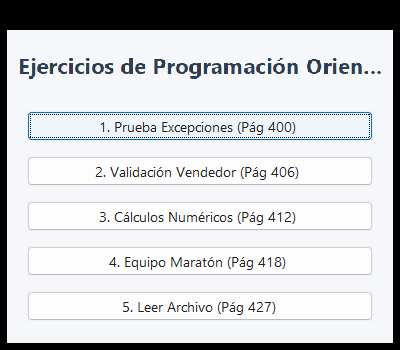
\includegraphics[width=0.55\textwidth]{imagenes/1}
    \caption{El menú principal que unifica e integra la Actividad 4.}
\end{figure}

\hrule
\bigskip

%----------------------------------------------------------------------------------------
%	EJERCICIO 1
%----------------------------------------------------------------------------------------
\section{Prueba de Excepciones (Pág. 400)}
\textbf{Requerimientos técnicos del ejercicio (Enunciado):}\\
\textit{Clase PruebaExcepciones:} ¿Cuál es el resultado de la ejecución del método \texttt{main} del programa? Determinar qué se imprime en pantalla. El programa debe contener un bloque principal con dos bloques \texttt{try} que generan excepciones. El primero genera una \texttt{ArithmeticException} mediante una división por cero (10000/0), y el segundo genera una \texttt{Exception} invocando un método \texttt{toString()} sobre un objeto instanciado como nulo. En ambos casos, se deben estructurar los bloques \texttt{catch} y \texttt{finally} y verificar el flujo de impresión.

\subsection{Interfaz de usuario}
A continuación se detalla la interfaz gráfica construida para la ejecución y visualización de la traza de excepciones en lugar de usar solo la consola. Se provee un botón para iniciar la simulación del error y un área de texto estilizada que muestra paso a paso las capturas de error y finalizadores.

\begin{figure}[H]
    \centering
    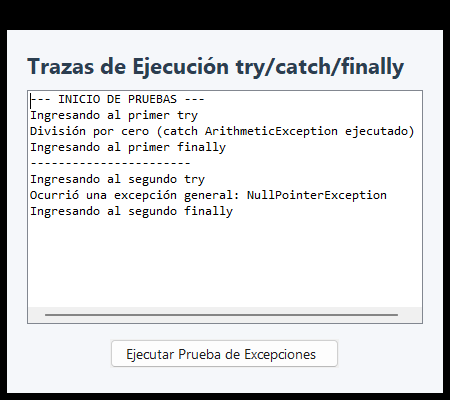
\includegraphics[width=0.55\textwidth]{imagenes/2}
    \caption{Ventana de visualización de Trazas de Excepciones tras la ejecución de las pruebas.}
\end{figure}

\subsection{Diagrama de clases}
\begin{figure}[H]
\begin{center}
\resizebox{0.9\textwidth}{!}{%
\begin{tikzpicture}[
  font=\sffamily,
  inheritance/.style={draw=inheritColor, line width=1.2pt, -{Triangle[open, length=10pt, width=12pt]}},
  association/.style={draw=assocColor, line width=0.8pt, -{Latex[length=6pt, width=7pt]}},
  label/.style={font=\scriptsize\sffamily, fill=white, inner sep=2pt, rounded corners=2pt, text=assocColor}
]
  \umlclass{Principal}{(0,0)}{3.0cm}{headerBlue}{Principal}{}{+main(String[])}
  \umlclass{Menu}{(4.5,0)}{5.0cm}{headerBlue}{VentanaPrincipalActividad4}{-btnEj1: JButton\\-btnEj2: JButton\\-btnEj3: JButton\\-btnEj4: JButton\\-btnEj5: JButton}{+VentanaPrincipalActividad4()}
  \umlclass{Ventana1}{(10.2,0)}{4.5cm}{headerBlue}{VentanaExcepciones}{-areaTexto: JTextArea}{+ejecutarPrueba()\\-imprimir(String)}
  
  \draw[association] (Principal.east) -- (Menu.west) node[label, midway, above] {Inicia};
  \draw[association] (Menu.east) -- (Ventana1.west) node[label, midway, above] {Abre};
\end{tikzpicture}%
}
\caption{Diagrama de clases para el ejercicio de Prueba de Excepciones.}
\end{center}
\end{figure}

\subsection{Casos de uso}
\begin{itemize}
    \item \textbf{Caso de Uso 1: Ejecutar Trazas de Excepción}
    \begin{itemize}
        \item \textbf{Actor:} Usuario.
        \item \textbf{Precondición:} La ventana \textit{Prueba Excepciones} debe estar desplegada.
        \item \textbf{Flujo Principal:} El usuario presiona el botón \textit{Ejecutar Prueba de Excepciones}. El sistema ejecuta internamente la división entera por cero y la referencia nula, captura las excepciones correspondientes (\texttt{ArithmeticException} y \texttt{Exception}) e imprime en pantalla el flujo paso a paso incluyendo las sentencias obligatorias de los bloques \texttt{finally}.
    \end{itemize}
\end{itemize}

\subsection{Link}
El código correspondiente a este ejercicio puede verificarse en:
\url{https://github.com/mateolikescats/POO/tree/main/Actividad_4/src/PruebaExcepciones}

\newpage

%----------------------------------------------------------------------------------------
%	EJERCICIO 2
%----------------------------------------------------------------------------------------
\section{Validación Vendedor (Pág. 406)}
\textbf{Requerimientos técnicos del ejercicio (Enunciado):}\\
\textit{Clase Vendedor:} Se requiere implementar una clase Vendedor que posee los siguientes atributos: nombre (tipo String), apellidos (tipo String) y edad (tipo int). La clase contiene un constructor que inicialice los atributos. Además, la clase posee los métodos:
\begin{itemize}
    \item \textbf{Imprimir}: muestra por pantalla los valores de sus atributos.
    \item \textbf{Verificar edad}: recibe como parámetro un valor entero que representa la edad del vendedor. Para que pueda desempeñar sus labores se requiere que sea mayor de edad (mayor de 18 años). Si esta condición no se cumple, se lanza una excepción de tipo \texttt{IllegalArgumentException} con el mensaje ``El vendedor debe ser mayor de 18 años''. Además, se evalúa si la edad se encuentra en el rango de 0 a 120, si no se cumple, se genera otra excepción de tipo \texttt{IllegalArgumentException} con el mensaje ``La edad no puede ser negativa ni mayor a 120''. Si la edad cumple estos requerimientos se puede instanciar el objeto.
\end{itemize}
Además, se requiere que los datos del vendedor se ingresen por teclado (en nuestro caso, a través de una GUI).

\subsection{Interfaz de usuario}
La GUI para la creación del vendedor cuenta con campos para ingresar el nombre, los apellidos y la edad del vendedor. Al pulsar el botón ``Crear y Validar'', se efectúa la validación solicitada y, si es correcta, se notifica el éxito. Si la edad está fuera de los rangos válidos, se captura la excepción correspondiente y se muestra en una alerta.

\begin{figure}[H]
    \centering
    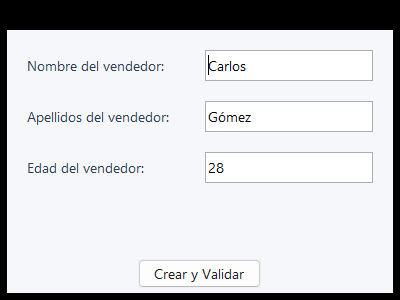
\includegraphics[width=0.55\textwidth]{imagenes/3}
    \caption{Ventana de registro y validación del Vendedor.}
\end{figure}

\subsection{Diagrama de clases}
\begin{figure}[H]
\begin{center}
\resizebox{0.75\textwidth}{!}{%
\begin{tikzpicture}[
  font=\sffamily,
  association/.style={draw=assocColor, line width=0.8pt, -{Latex[length=6pt, width=7pt]}},
  label/.style={font=\scriptsize\sffamily, fill=white, inner sep=2pt, rounded corners=2pt, text=assocColor}
]
  \umlclass{Ventana2}{(0,0)}{4.5cm}{headerBlue}{VentanaVendedor}{-campoNombre: JTextField\\-campoApellidos: JTextField\\-campoEdad: JTextField}{+crearVendedor()}
  \umlclass{Vendedor}{(6.0,0)}{4.5cm}{headerGreen}{Vendedor}{-nombre: String\\-apellidos: String\\-edad: int}{+Vendedor(String, String, int)\\-verificarEdad(int)\\+toString()}
  
  \draw[association] (Ventana2.east) -- (Vendedor.west) node[label, midway, above] {Instancia};
\end{tikzpicture}%
}
\caption{Diagrama de clases para el ejercicio de Validación del Vendedor.}
\end{center}
\end{figure}

\subsection{Casos de uso}
\begin{itemize}
    \item \textbf{Caso de Uso 1: Crear Vendedor con Datos Válidos}
    \begin{itemize}
        \item \textbf{Actor:} Usuario.
        \item \textbf{Flujo Principal:} El usuario digita el nombre, los apellidos y una edad dentro del rango [18, 120] y hace clic en \textit{Crear y Validar}. El sistema valida e instancia el \texttt{Vendedor}, mostrando los datos con el método \texttt{toString()}.
    \end{itemize}
    \item \textbf{Caso de Uso 2: Intentar Crear Vendedor Menor de Edad o Edad Fuera de Rango}
    \begin{itemize}
        \item \textbf{Actor:} Usuario.
        \item \textbf{Flujo Alternativo:} El usuario ingresa una edad menor de 18 años, negativa, o mayor a 120. El sistema interrumpe la lógica lanzando \texttt{IllegalArgumentException} y el controlador notifica el error formal en pantalla.
    \end{itemize}
\end{itemize}

\subsection{Link}
El código correspondiente a este ejercicio puede verificarse en:
\url{https://github.com/mateolikescats/POO/tree/main/Actividad_4/src/Vendedor}

\newpage

%----------------------------------------------------------------------------------------
%	EJERCICIO 3
%----------------------------------------------------------------------------------------
\section{Cálculos Numéricos (Pág. 412)}
\textbf{Requerimientos técnicos del ejercicio (Enunciado):}\\
\textit{Clase CálculosNuméricos:} Se requiere definir una clase que realice las siguientes operaciones:
\begin{itemize}
    \item Calcular el \textbf{logaritmo neperiano} recibiendo un valor \texttt{double} como parámetro. Este método debe ser estático. Si el valor no es positivo se genera una excepción aritmética.
    \item Calcular la \textbf{raíz cuadrada} recibiendo un valor \texttt{double} como parámetro. Este método debe ser estático. Si el valor no es positivo se genera una excepción aritmética.
    \item Se debe crear un método \texttt{main} que utilice dichos métodos ingresando un valor por teclado.
\end{itemize}

\subsection{Interfaz de usuario}
La interfaz gráfica de usuario permite la captura del valor numérico e incorpora dos botones autónomos para activar por separado los cálculos de logaritmo y raíz cuadrada. El resultado o error aritmético se muestra en la etiqueta de resultados o como alerta interactiva.

\begin{figure}[H]
    \centering
    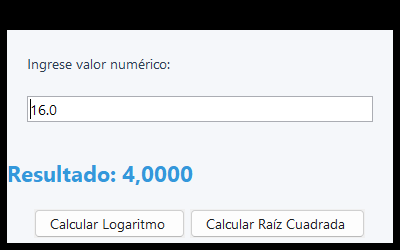
\includegraphics[width=0.55\textwidth]{imagenes/4}
    \caption{Ventana para realizar Cálculos Numéricos avanzados con control de excepciones.}
\end{figure}

\subsection{Diagrama de clases}
\begin{figure}[H]
\begin{center}
\resizebox{0.75\textwidth}{!}{%
\begin{tikzpicture}[
  font=\sffamily,
  association/.style={draw=assocColor, line width=0.8pt, -{Latex[length=6pt, width=7pt]}},
  label/.style={font=\scriptsize\sffamily, fill=white, inner sep=2pt, rounded corners=2pt, text=assocColor}
]
  \umlclass{Ventana3}{(0,0)}{4.8cm}{headerBlue}{VentanaCalculos}{-campoValor: JTextField\\-lblResultado: JLabel}{+calcularLogaritmo()\\+calcularRaiz()}
  \umlclass{Calculos}{(6.0,0)}{5.0cm}{headerGreen}{CalculosNumericos}{}{+calcularLogaritmoNeperiano(double)\$\\+calcularRaizCuadrada(double)\$}
  
  \draw[association] (Ventana3.east) -- (Calculos.west) node[label, midway, above] {Utiliza};
\end{tikzpicture}%
}
\caption{Diagrama de clases para el ejercicio de Cálculos Numéricos.}
\end{center}
\end{figure}

\subsection{Casos de uso}
\begin{itemize}
    \item \textbf{Caso de Uso 1: Calcular Operación con Valor Positivo}
    \begin{itemize}
        \item \textbf{Actor:} Usuario.
        \item \textbf{Flujo Principal:} El usuario escribe un número real positivo y presiona cualquiera de los botones de cálculo. El sistema computa la raíz o el logaritmo de forma estática y muestra el resultado en el label inferior.
    \end{itemize}
    \item \textbf{Caso de Uso 2: Gestionar Excepciones Numéricas}
    \begin{itemize}
        \item \textbf{Actor:} Usuario.
        \item \textbf{Flujo Alternativo:} Si el número ingresado es negativo o posee texto, el sistema lanza y captura una \texttt{ArithmeticException} o un \texttt{NumberFormatException}, evitando el colapso del sistema y alertando al usuario visualmente.
    \end{itemize}
\end{itemize}

\subsection{Link}
El código correspondiente a este ejercicio puede verificarse en:
\url{https://github.com/mateolikescats/POO/tree/main/Actividad_4/src/CalculosNumericos}

\newpage

%----------------------------------------------------------------------------------------
%	EJERCICIO 4
%----------------------------------------------------------------------------------------
\section{Equipo Maratón (Pág. 418)}
\textbf{Requerimientos técnicos del ejercicio (Enunciado):}\\
\textit{Clase EquipoMaratónProgramación:} Un equipo desea participar en una maratón. Tiene los atributos: Nombre del equipo, Universidad, Lenguaje de programación, y Tamaño del equipo. El equipo está conformado por varios programadores (mínimo dos y máximo tres), cada uno con nombre y apellidos.
Se requieren los siguientes métodos:
\begin{itemize}
    \item Un método para determinar si el equipo está completo.
    \item Un método para añadir programadores al equipo. Si el equipo está lleno se debe imprimir la excepción correspondiente.
    \item Un método para validar los atributos nombre y apellidos de un programador para que reciban \textbf{solo texto}. Si se reciben datos numéricos se debe generar la excepción correspondiente. Además, no se permiten campos con una longitud igual o superior a 20 caracteres.
\end{itemize}
\textit{Ejercicios propuestos (Pág 425):} Como adición formativa en la actividad, el libro propone desarrollar también una validación estricta de contraseña (mínimo 8 caracteres, sin espacios, con mayúsculas, un número y un carácter especial, capturando los errores mediante excepciones). En nuestra interfaz, las aserciones sobre atributos cubren estos lineamientos aplicando lógica de validación similar sobre los nombres de los miembros del equipo.

\subsection{Interfaz de usuario}
La ventana está dividida en dos etapas secuenciales: primero se crea la estructura del equipo y luego se habilitan los campos para ir agregando iterativamente cada programador a la lista, comprobando caracteres ilícitos y el desbordamiento de capacidad.

\begin{figure}[H]
    \centering
    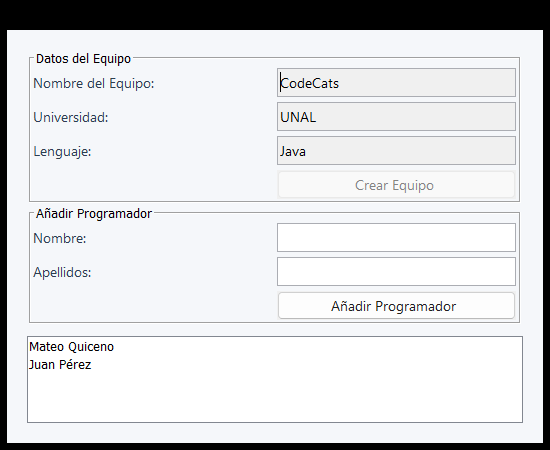
\includegraphics[width=0.60\textwidth]{imagenes/5}
    \caption{Ventana de gestión y registro de miembros del Equipo Maratón.}
\end{figure}

\subsection{Diagrama de clases}
\begin{figure}[H]
\begin{center}
\resizebox{0.95\textwidth}{!}{%
\begin{tikzpicture}[
  font=\sffamily,
  association/.style={draw=assocColor, line width=0.8pt, -{Latex[length=6pt, width=7pt]}},
  label/.style={font=\scriptsize\sffamily, fill=white, inner sep=2pt, rounded corners=2pt, text=assocColor}
]
  \umlclass{Ventana4}{(0,0)}{4.5cm}{headerBlue}{VentanaEquipo}{-txtNomEquipo: JTextField\\-txtUniversidad: JTextField\\-txtLenguaje: JTextField\\-txtNomProg: JTextField\\-txtApeProg: JTextField}{+crearEquipo()\\+anadirProgramador()}
  \umlclass{Equipo}{(5.8,0)}{5.2cm}{headerGreen}{EquipoMaratonProgramacion}{-nombreEquipo: String\\-universidad: String\\-lenguajeProgramacion: String\\-programadores: Programador[]\\-tamañoEquipo: int}{+EquipoMaratonProgramacion()\\+estaLleno(): boolean\\+añadir(Programador)\\+validarCampo(String)\$}
  \umlclass{Prog}{(12.2,0)}{3.8cm}{headerGreen}{Programador}{-nombre: String\\-apellidos: String}{+Programador(String, String)\\+toString()}
  
  \draw[association] (Ventana4.east) -- (Equipo.west) node[label, midway, above] {Crea};
  \draw[association] (Equipo.east) -- (Prog.west) node[label, midway, above] {Contiene};
\end{tikzpicture}%
}
\caption{Diagrama de clases para el ejercicio de Equipo Maratón de Programación.}
\end{center}
\end{figure}

\subsection{Casos de uso}
\begin{itemize}
    \item \textbf{Caso de Uso 1: Crear Equipo e Inscribir Integrantes}
    \begin{itemize}
        \item \textbf{Actor:} Usuario.
        \item \textbf{Flujo Principal:} El usuario inicializa el equipo y añade hasta 3 programadores. El sistema valida las longitudes ($\le$ 20) y la ausencia de dígitos en los nombres, lanzando excepciones si no cumplen la política estructural.
    \end{itemize}
    \item \textbf{Caso de Uso 2: Controlar Exceso de Capacidad}
    \begin{itemize}
        \item \textbf{Actor:} Sistema.
        \item \textbf{Flujo Alternativo:} Intentar añadir un 4to integrante ocasiona que \texttt{añadir()} genere una excepción de capacidad agotada, impidiendo la modificación del arreglo interno.
    \end{itemize}
\end{itemize}

\subsection{Link}
El código correspondiente a este ejercicio puede verificarse en:
\url{https://github.com/mateolikescats/POO/tree/main/Actividad_4/src/EquipoMaraton}

\newpage

%----------------------------------------------------------------------------------------
%	EJERCICIO 5
%----------------------------------------------------------------------------------------
\section{Leer Archivo (Pág. 427)}
\textbf{Requerimientos técnicos del ejercicio (Enunciado):}\\
\textit{Clase LeerArchivo:} Se tiene un archivo de texto denominado \texttt{prueba.txt} en una cierta localización en un sistema de archivos. Se requiere desarrollar un programa que lea dicho archivo de texto utilizando un flujo de bytes que muestre los contenidos del archivo en pantalla. Para esto, se debe instanciar un flujo con \texttt{FileInputStream}, enlazarlo con \texttt{InputStreamReader} y finalmente utilizar \texttt{BufferedReader} para efectuar la lectura con \texttt{readLine()} asegurando la captura correcta de \texttt{IOException} si el documento es inaccesible o si el flujo falla.

\subsection{Interfaz de usuario}
La ventana del lector cuenta con un selector nativo de Windows (\texttt{JFileChooser}) activado por botón. El contenido se carga dinámicamente y se imprime en el área de texto protegida.

\begin{figure}[H]
    \centering
    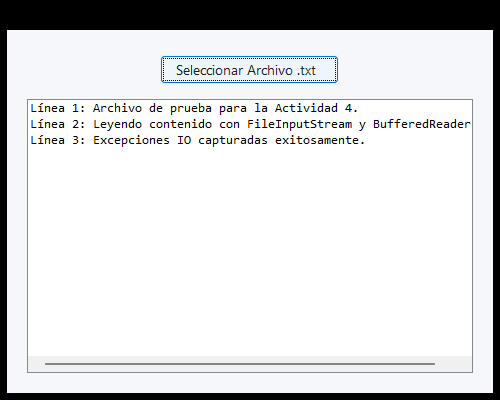
\includegraphics[width=0.55\textwidth]{imagenes/6}
    \caption{Ventana del Lector de Archivos de Texto con control de fallos I/O.}
\end{figure}

\subsection{Diagrama de clases}
\begin{figure}[H]
\begin{center}
\resizebox{0.35\textwidth}{!}{%
\begin{tikzpicture}[
  font=\sffamily
]
  \umlclass{Ventana5}{(0,0)}{4.5cm}{headerBlue}{VentanaLeerArchivo}{-areaTexto: JTextArea}{+leerArchivo()}
\end{tikzpicture}%
}
\caption{Diagrama de clases para el ejercicio de Lectura de Archivos.}
\end{center}
\end{figure}

\subsection{Casos de uso}
\begin{itemize}
    \item \textbf{Caso de Uso 1: Seleccionar y Leer Archivo de Texto}
    \begin{itemize}
        \item \textbf{Actor:} Usuario.
        \item \textbf{Flujo Principal:} El usuario selecciona un archivo \texttt{.txt} a través de la ventana de diálogo, el buffer extrae el contenido de bytes traduciéndolo a Unicode y este se renderiza línea por línea en pantalla.
    \end{itemize}
    \item \textbf{Caso de Uso 2: Fallo de Lectura (IOException)}
    \begin{itemize}
        \item \textbf{Actor:} Sistema.
        \item \textbf{Flujo Alternativo:} Si el flujo falla por inaccesibilidad o daño del disco, el sistema detecta \texttt{IOException} y advierte al usuario de manera controlada.
    \end{itemize}
\end{itemize}

\subsection{Link}
El código correspondiente a este ejercicio puede verificarse en:
\url{https://github.com/mateolikescats/POO/tree/main/Actividad_4/src/LeerArchivo}

\newpage

%----------------------------------------------------------------------------------------
%	CONCLUSION
%----------------------------------------------------------------------------------------
\section{Conclusión}
Esta actividad sirvió para entender a fondo el ciclo de vida de los errores del sistema y la captura inteligente de excepciones en Java, delegando la responsabilidad de procesamiento desde las clases de negocio puras hacia los controladores gráficos de las ventanas. El uso de bloques \texttt{try-catch-finally} y el lanzamiento explícito de excepciones de usuario permiten modelar restricciones y resguardar la estabilidad del software, evitando caídas abruptas y transformando condiciones críticas de error en notificaciones dinámicas de cara al usuario final. Adicionalmente, se logró implementar correctamente arquitecturas de IO para lectura segura de archivos.

\end{document}
